\documentclass[letterpaper]{article}
\usepackage{natbib,alifeconf}
\usepackage{amsmath,amssymb,amsthm}
\usepackage{booktabs,graphicx,microtype}
\usepackage[hidelinks]{hyperref}

\graphicspath{{figures/}{../outputs/alife_2026/editable_figures/}{../poster/figures/}}
\setlength{\textfloatsep}{7pt plus 1pt minus 1pt}
\setlength{\floatsep}{6pt plus 1pt minus 1pt}
\setlength{\abovecaptionskip}{3pt}
\setlength{\belowcaptionskip}{0pt}

\newtheorem{theorem}{Theorem}
\newtheorem{proposition}[theorem]{Proposition}

\DeclareMathOperator*{\argmin}{arg\,min}
\newcommand{\bs}{\mathbf{s}}
\newcommand{\bD}{\mathbf{D}}
\newcommand{\bx}{\mathbf{x}}
\newcommand{\NML}{\operatorname{NML}}
\newcommand{\NLL}{\operatorname{NLL}}
\newcommand{\Hb}{H_b}

\title{Selecting Relative-Periodic Domains in Cellular Automaton Spacetime with Bernoulli NML}

\author{Anonymous$^{1}$ \\
\mbox{}\\
$^1$Anonymous Affiliation \\
anonymous@example.com}

\begin{document}
\maketitle

\begin{abstract}
Cellular automata often form broad periodic domains together with interfaces, defects, and particle-like activity. We introduce a fast global front end for that setting: scan relative-periodic templates, fit each template by majority vote on orbit classes, and return both a selected background scaffold and the residual mask that the scaffold does not explain. The Bernoulli normalized maximum likelihood (NML) score makes the comparison complexity-aware, preventing the period inflation that occurs with raw defect minimization and Bernoulli likelihood alone. Across 1D, 2D, and 3D examples, the selected scaffold usually stabilizes quickly, while 2D surveys show that most Life-like rules stay at low period and only a small number reveal longer periodic organization at larger horizons. The same decomposition isolates structured residuals in named rules such as Diamoeba, Maze with Mice, and S37/B11, where the residual mask is sparse but visibly organized rather than featureless noise. The supporting theory explains why higher-period templates overfit along refinement chains and why candidates with worse asymptotic fit are eventually excluded. The result is a scalable way to generate domain hypotheses and defect masks for downstream ALIFE analysis.
\end{abstract}

%======================================================================
\section{Introduction}
%======================================================================

Cellular automata (CA) frequently produce spacetime patterns in which broad regular domains coexist with defects, interfaces, and particle-rich activity. For ALIFE work, those domains matter because they provide the background against which coherent structures become visible. A practical problem follows immediately: given a finite spacetime, which global periodic organization best explains it, and what structure remains once that organization is removed?

Two established traditions address nearby questions. Computational mechanics and local causal-state methods recover local statistical structure and can identify domains, particles, and interactions in rich detail \citep{crutchfield1997,hanson1992,rupe2018,shalizi2006}. Survey-oriented and compression-oriented work instead emphasize broad rule catalogs and low-cost global summaries \citep{packard1985,boccara1999,zenil2010}. The method here is meant as a middle ground. It does not replace local structure reconstruction. Instead it provides a global front end that can be applied cheaply across many rules, yielding a compact domain hypothesis together with a residual mask that highlights where richer local analysis is likely to pay off.

A candidate period $p$ and shift $\bs$ induce a relative-periodic model class. Fitting that candidate reduces to a majority vote on orbit classes, producing a background scaffold $B^*(p,\bs)$ and residual mask $M = U \oplus B^*(p,\bs)$. Candidates are compared with a Bernoulli NML score that balances orbit-wise fit against model complexity. The resulting selector is fast enough for survey use, while still admitting theorem-level analysis of overcapacity and stabilization.

Concretely, the paper contributes a relative-periodic CA model family, an orbit-class fitting rule that runs in $O(|U|)$ time per candidate, a complexity-aware selector that avoids systematic period inflation, a compact stabilization theorem for finite candidate families, and cross-dimensional evidence that the scaffold-plus-residual decomposition is useful for CA structure discovery. The paper's claim is deliberately modest: the selected period is a global explanatory scaffold, not a complete account of particles or interactions.

\begin{figure*}[t]
    \centering
    
\includegraphics[width=0.92\textwidth]{algorithm_detailed.pdf}
    \caption{Algorithm sketch. A candidate period/shift pair induces an orbit partition of the observed spacetime. Majority vote on each orbit gives the nearest relative-periodic background $B^*(p,\bs)$, the residual mask is $M = U \oplus B^*(p,\bs)$, and Bernoulli NML compares candidates by orbit-wise fit plus complexity.}
    \label{fig:algorithm}
\end{figure*}

%======================================================================
\section{Method}
%======================================================================

\paragraph{Relative-periodic candidates.}
For a binary spacetime $U \in \{0,1\}^{T \times D_1 \times \cdots \times D_n}$, period $p \geq 1$, and shift $\bs \in \mathbb{Z}^n$, the relative-periodic model class $\mathcal{B}(p,\bs)$ consists of fields $B$ satisfying
\[
B[t+p,\bx+\bs \bmod \bD] = B[t,\bx].
\]
The corresponding spacetime translation partitions the observation into orbit classes $\{O_j\}_{j=1}^{k}$ with $k = p \prod_i D_i$. A candidate background therefore assigns one bit to each orbit class.

\begin{proposition}[Orbitwise fitting]\label{prop:projection}
For a fixed candidate $(p,\bs)$, the Hamming-optimal background in $\mathcal{B}(p,\bs)$ is obtained by majority vote on each orbit class. If $n_j^{(1)}$ and $n_j^{(0)}$ denote the number of ones and zeros in class $O_j$, then the minimum residual count is $\sum_j \min(n_j^{(0)}, n_j^{(1)})$.
\end{proposition}

This orbit-class reduction is the computational core of the method. Once the orbit partition is known, fitting is a single pass over the data.

\paragraph{Bernoulli NML score.}
Each orbit class becomes a Bernoulli estimation problem with empirical parameter $\hat{\theta}_j = n_j^{(1)}/n_j$, where $n_j = |O_j|$. We score a candidate by
\[
\NML(p,\bs) = \sum_j n_j \Hb(\hat{\theta}_j) + \frac{1}{2}\sum_j \log_2 n_j,
\]
where the first term is Bernoulli negative log-likelihood and the second is the asymptotic NML complexity penalty for Bernoulli families \citep{grunwald2007,shtarkov1987}. The selector minimizes this score over the scanned period/shift family.

\begin{theorem}[Refinement and overcapacity]\label{thm:refinement}
If $(p_2,\bs_2)$ is a velocity-matched multiple of $(p_1,\bs_1)$, then the orbit partition under $(p_2,\bs_2)$ refines the partition under $(p_1,\bs_1)$. Consequently both optimal residual count and Bernoulli NLL are non-increasing along that chain.
\end{theorem}

The practical message of Theorem~\ref{thm:refinement} is that raw defect minimization and raw Bernoulli likelihood systematically overselect larger templates whenever refinement is available. Complexity control is therefore necessary, not cosmetic.

\begin{theorem}[Stabilization]\label{thm:stabilization}
Let $\mathcal{C}$ be a finite candidate set and let $N(T)$ denote the number of observed sites. If the orbit-class frequencies for each candidate converge as the observation horizon grows, then
\[
\NML(c,T) = \lambda_c N(T) + \frac{k_c}{2}\log_2 T + o(N(T)),
\]
where $\lambda_c$ is the candidate's asymptotic per-site Bernoulli fit rate and $k_c$ is its number of orbit classes. Every candidate with $\lambda_c$ above the minimum is eventually excluded, and if the minimum rate is unique then the selector locks to a single winner.
\end{theorem}

This is the standard MDL/NML rate-separation argument specialized to relative-periodic orbit models: asymptotic fit differences grow linearly in data size, while complexity grows only logarithmically. It supports treating the selected candidate as the best global explanation of the observed spacetime. That need not coincide with a physicist's ``true'' background period: if the residual itself contains periodic organization, a larger template can absorb it; when the background is exactly periodic, the smaller true period wins because matched multiples pay higher complexity.

%======================================================================
\section{Results}
%======================================================================

\subsection{Representative Decompositions}

\begin{figure*}[t]
  \centering
  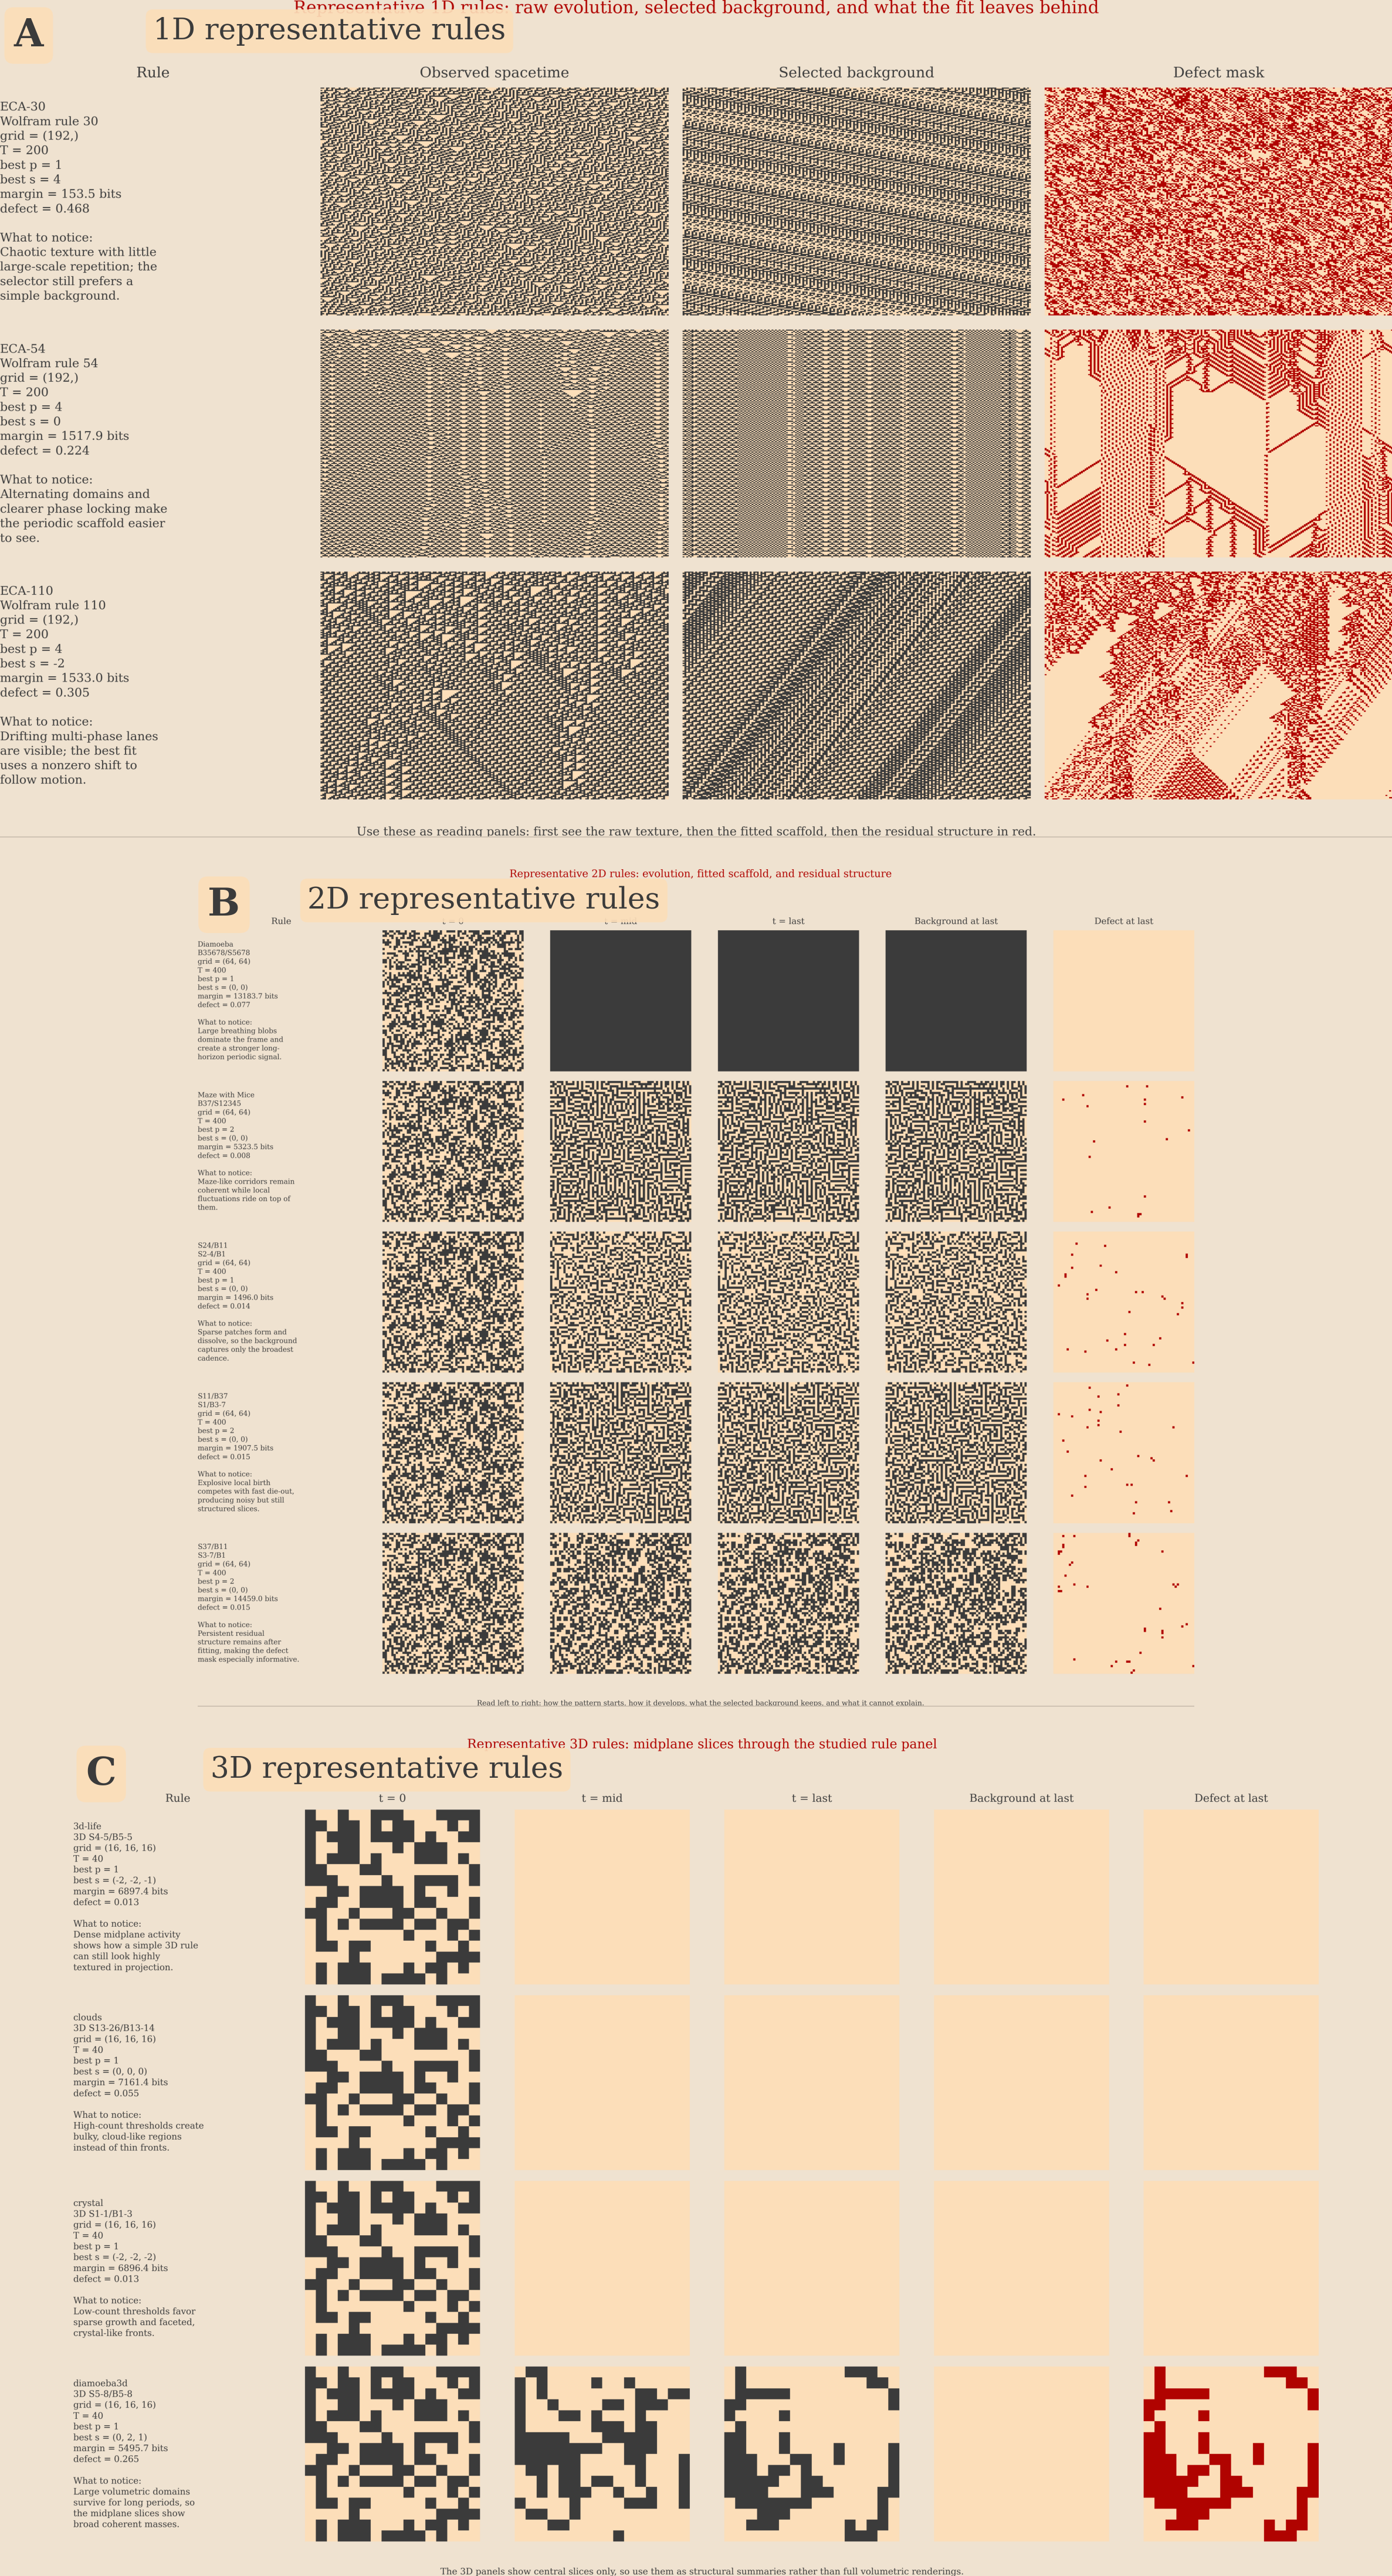
\includegraphics[width=\textwidth,height=0.78\textheight,keepaspectratio]{alife_representative_rules.png}
  \caption{Representative decompositions across 1D, 2D, and 3D. The same selector extracts a broad relative-periodic scaffold and the residual mask left after subtraction. In the focal 2D cases, the residual remains sparse but visibly structured rather than collapsing to featureless noise.}
  \label{fig:representative}
\end{figure*}

Figure~\ref{fig:representative} shows the main empirical use case. Across dimensions, the selector removes the broad regular scaffold while leaving behind the defects and interfaces that the scaffold does not explain. In the 2D named rules that matter most for ALIFE interpretation, Diamoeba (B35678/S5678) and Maze with Mice (B37/S12345) produce low-period scaffolds with concentrated residual masks, while S37/B11 retains a visibly organized residual population even after the background is removed.

The 1D examples provide the same kind of scaffold extraction under joint shift-period optimization: Rule~54 locks to period~4, Rule~110 passes through a short transient and then locks to period~4 with shift $-2$, and Rule~30 remains at period~1. In 3D, the tested diamoeba rule shows an analogous decomposition once the early small-sample transient disappears.

\subsection{Why the Penalty Matters}

\begin{figure}[t]
    \centering
    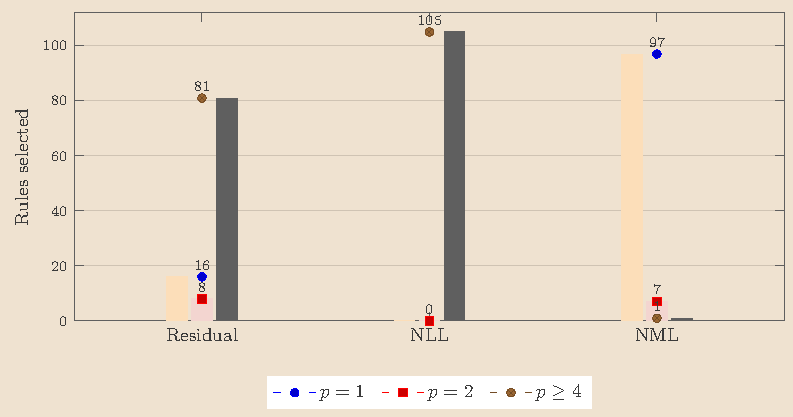
\includegraphics[width=0.98\linewidth]{selector_ablation_tikz.pdf}
    \caption{Selector ablation on nontrivial Life-like rules at $T=100$. Raw residual minimization and Bernoulli NLL are pulled toward larger periods along refinement chains. Bernoulli NML prevents that period inflation and concentrates selections at low period.}
    \label{fig:ablation}
\end{figure}

Figure~\ref{fig:ablation} is the key practical argument for NML. On the 105 nontrivial Life-like rules at $T=100$, Bernoulli NLL selects the largest tested period in every case. Bernoulli NML instead selects period~1 for 97 rules, period~2 for 7 rules, and period~8 for 1 rule. Residual minimization shows the same upward pull toward more expressive templates. The complexity term is therefore doing real work: it prevents the selector from confusing refinement capacity with meaningful periodic structure.

\subsection{Cross-Dimensional Behavior and 2D Surveys}

We surveyed all 106 named Life-like rules from the LifeWiki on a $64 \times 64$ torus with periods 1--8 and shifts $\pm 2$. Most nontrivial rules remain low period at both horizons we tested. Only four rules change period between $T=100$ and $T=400$: Diamoeba and Maze with Mice move from period~1 to period~2, B017/S01 moves from period~2 to period~4, and Serviettes (B234/S) drops from period~2 to period~1 as a transient disappears. Fredkin (B1357/S02468) is the only named rule that reaches period~8.

\begin{table}[t]
\centering
\caption{Life-like survey period distribution (nontrivial rules only).}
\label{tab:lifewiki}
\begin{tabular}{lcc}
\toprule
Period & $T=100$ & $T=400$ \\
\midrule
$p=1$ & 97 & 94 \\
$p=2$ & 7 & 7 \\
$p=4$ & 0 & 1 \\
$p=8$ & 1 & 1 \\
\midrule
Nontrivial & 105 / 106 & 103 / 106 \\
\bottomrule
\end{tabular}
\end{table}

The same stabilization picture appears across dimensions, but with different transient behaviors. In 2D persistent-residual rules, longer horizons can reveal additional periodic structure before the selector locks. In 3D diamoeba3d, the initial period~6 selection is a small-sample artifact and period~1 takes over by $T=40$ with growing margin. These cases match the theoretical picture: the selector changes when longer observation windows uncover fit improvements strong enough to beat the logarithmic complexity penalty.

\begin{table}[t]
\centering
\caption{Compact cross-dimensional summary of the selected scaffold behavior.}
\label{tab:summary}
\small
\begin{tabular}{p{0.21\linewidth}p{0.67\linewidth}}
\toprule
Setting & Main observation \\
\midrule
1D ECA 30/54/110 & Rule~54 locks to period~4, Rule~110 locks to period~4 with shift $-2$ after a short transient, and Rule~30 remains at period~1. \\
2D Life-like survey & At $T=400$, 94 of 103 nontrivial named rules select period~1; only 9 named rules select period $>1$. \\
2D focal persistent-residual rules & S24/B11 and S37/B11 move to period~2, S11/B37 moves to period~4, and all retain organized residual structure after subtraction. \\
3D diamoeba3d & A short small-sample transient favors period~6, but the selector stabilizes to period~1 by $T=40$. \\
\bottomrule
\end{tabular}
\end{table}

\subsection{Structured Residuals as the ALIFE Payoff}

The main ALIFE value of the method is not just period selection. The selected background acts as a domain hypothesis, and the residual mask highlights where particles, interfaces, and other coherent departures remain. In Diamoeba and Maze with Mice the residual is sparse but clearly localized. In S37/B11, the residual remains organized under stronger checks: the same rule continues to show persistent structured defects at 400 steps, across 10 seeds, and at grid sizes up to $192 \times 192$. That makes the decomposition useful as a survey-scale triage tool. It tells us which rules, horizons, and spatial regions merit the heavier cost of local causal-state or particle-level analysis.

%======================================================================
\section{Discussion}
%======================================================================

This method is deliberately modest. It is complementary to computational mechanics rather than a replacement for it. The output is a compact global scaffold and a residual mask, not a full account of interaction structure. What it buys in exchange is scale: the same orbit-class computation can be applied across many rules and across 1D, 2D, and 3D settings without changing the basic pipeline.

The theory explains why that pipeline behaves sensibly. Majority-vote fitting gives a cheap global projection, refinement explains why unpenalized selectors overfit, and the stabilization result explains why longer observation windows typically reduce ambiguity rather than increase it. The main limitations are equally clear: the selector chooses the best-compressing global explanation, not necessarily a unique physical background period, and the residual mask indicates where structure is but not how it interacts. The next steps are direct comparisons with local causal states, component tracking within the residual mask, and exact finite-sample NML normalizers. All experiments and figures reported here come from the same open-source project repository and reuse the existing 1D, 2D, and 3D survey outputs rather than introducing new experiments.

%======================================================================
\section{Conclusion}
%======================================================================

Bernoulli NML selection of relative-periodic templates provides a scalable front end for CA structure discovery. It yields a domain hypothesis and residual mask, avoids period inflation, and supports rapid comparison of periodic explanations across rules and dimensions. The supporting theory explains why complexity control is necessary and why the selected scaffold usually stabilizes as the observation window grows.

For ALIFE, the main payoff is practical. The method makes it easier to screen many rules, isolate where coherent departures from a broad background remain, and focus richer local analyses on the cases where they are most likely to be informative.

\footnotesize
\bibliographystyle{apalike}
\begin{thebibliography}{9}

\bibitem[Boccara and Roger, 1999]{boccara1999}
Boccara, N. and Roger, M. (1999).
Totalistic two-dimensional cellular automata exhibiting global periodic behavior.
\emph{Int.\ J.\ Modern Physics~C}, 10(6):1051--1066.

\bibitem[Crutchfield and Hanson, 1997]{crutchfield1997}
Crutchfield, J.~P. and Hanson, J.~E. (1997).
Computational mechanics of cellular automata: An example.
\emph{Physica D}, 103:169--189.

\bibitem[Gr{\"u}nwald, 2007]{grunwald2007}
Gr{\"u}nwald, P. (2007).
\emph{The Minimum Description Length Principle}.
MIT Press.

\bibitem[Hanson and Crutchfield, 1992]{hanson1992}
Hanson, J.~E. and Crutchfield, J.~P. (1992).
The attractor-basin portrait of a cellular automaton.
\emph{J.\ Statistical Physics}, 66:1415--1462.

\bibitem[Packard and Wolfram, 1985]{packard1985}
Packard, N.~H. and Wolfram, S. (1985).
Two-dimensional cellular automata.
\emph{J.\ Statistical Physics}, 38:901--946.

\bibitem[Rupe and Crutchfield, 2018]{rupe2018}
Rupe, A. and Crutchfield, J.~P. (2018).
Local causal states and discrete coherent structures.
\emph{Chaos}, 28:075312.

\bibitem[Shalizi et~al., 2006]{shalizi2006}
Shalizi, C.~R., Haslinger, R., Rouquier, J.-B., Klinkner, K.~L., and Moore, C. (2006).
Automatic filters for the detection of coherent structure in spatiotemporal systems.
\emph{Physical Review~E}, 73:036104.

\bibitem[Shtarkov, 1987]{shtarkov1987}
Shtarkov, Y. (1987).
Universal sequential coding of single messages.
\emph{Problems of Information Transmission}, 23:3--17.

\bibitem[Zenil, 2010]{zenil2010}
Zenil, H. (2010).
Compression-based investigation of the dynamical properties of cellular automata and other systems.
\emph{Complex Systems}, 19(1):1--28.

\end{thebibliography}

\end{document}
